%!TEX root = ../paper.tex

% Small differences in anisotropy  
	% Where are the differeneces largest -> plots
	% Kernel is sensitive to spurious structure in the data

% Highest anisotropy of noise component 
	% Kernel 'catches' spurious structures in noise -> increase K.

% 	  Denser component -> higher anisotropy of kernels
% AND Higher anistropy in component -> higer anisotropy in associated kernels
% AND Denser comonent -> lower MSE
	% Introduce the dataset A1 and A2, same anisotropy different density, what do we observe, what does it say about this correlation.

% Lack of difference in anisotropy between F3 and B3 in orange (‘Trivariate Gaussian 3’) component. 


	\begin{figure}
		\centering
		\begin{subfigure}{0.23\textwidth}
			\centering
			\includegraphics[keepaspectratio=true, width=\textwidth, height=0.23\textheight]{discussion/img/ferdosi_1_60000_anisotropy.png}
			\caption{Dataset \ferdosiOne}
			\label{fig:discussion:anisotropy:ferdosi1}
		\end{subfigure}
		\begin{subfigure}{0.23\textwidth}
			\centering
			\includegraphics[keepaspectratio=true, width=\textwidth, height=0.23\textheight]{discussion/img/ferdosi_1_60000_anisotropy.png}
			\caption{Dataset \baakmanOne}
			\label{fig:discussion:anisotropy:baakman1}
		\end{subfigure}	
		\begin{subfigure}{0.23\textwidth}
			\centering
			\includegraphics[keepaspectratio=true, width=\textwidth, height=0.23\textheight]{discussion/img/baakman_4_60000_anisotropy.png}
			\caption{Dataset \baakmanFour}
			\label{fig:discussion:anisotropy:baakman4}
		\end{subfigure}		
		\begin{subfigure}{0.23\textwidth}
			\centering
			\includegraphics[keepaspectratio=true, width=\textwidth, height=0.23\textheight]{discussion/img/baakman_5_60000_anisotropy.png}
			\caption{Dataset \baakmanFive}
			\label{fig:discussion:anisotropy:baakman5}
		\end{subfigure}			
		\caption{Scatter plot of the data sets
			\subref{fig:discussion:anisotropy:ferdosi1} \ferdosiOne, %
			\subref{fig:discussion:anisotropy:baakman1} \baakmanOne, %
			\subref{fig:discussion:anisotropy:baakman4} \baakmanFour, and %
			\subref{fig:discussion:anisotropy:baakman5} \baakmanFive. %
			The points whose anisotropy lies in the \nth{90} percentile are shown larger and in the color of the component they were drawn from.}
		\label{fig:discussion:anisotropy:singleSphere}
	\end{figure}

	\begin{figure}
		\centering
		\begin{subfigure}{0.23\textwidth}
			\centering
			\includegraphics[keepaspectratio=true, width=\textwidth, height=0.23\textheight]{discussion/img/ferdosi_2_60000_anisotropy.png}
			\caption{Dataset \ferdosiTwo}
			\label{fig:discussion:anisotropy:ferdosi2}
		\end{subfigure}
		\begin{subfigure}{0.23\textwidth}
			\centering
			\includegraphics[keepaspectratio=true, width=\textwidth, height=0.23\textheight]{discussion/img/baakman_2_60000_anisotropy.png}
			\caption{Dataset \baakmanTwo}
			\label{fig:discussion:anisotropy:baakman2}
		\end{subfigure}	
		\begin{subfigure}{0.23\textwidth}
			\centering
			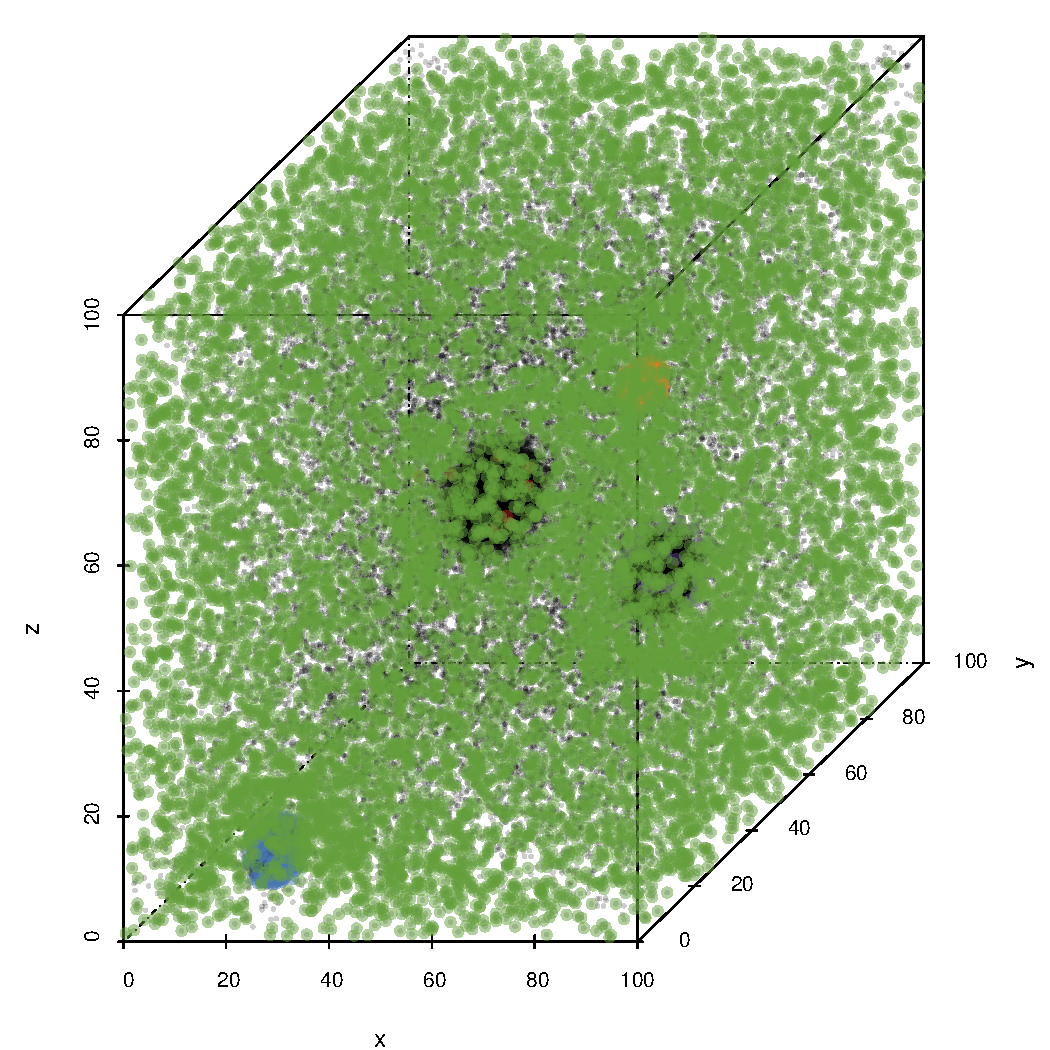
\includegraphics[keepaspectratio=true, width=\textwidth, height=0.23\textheight]{discussion/img/ferdosi_3_120000_anisotropy.png}
			\caption{Dataset \ferdosiThree}
			\label{fig:discussion:anisotropy:ferdosi3}
		\end{subfigure}		
		\begin{subfigure}{0.23\textwidth}
			\centering
			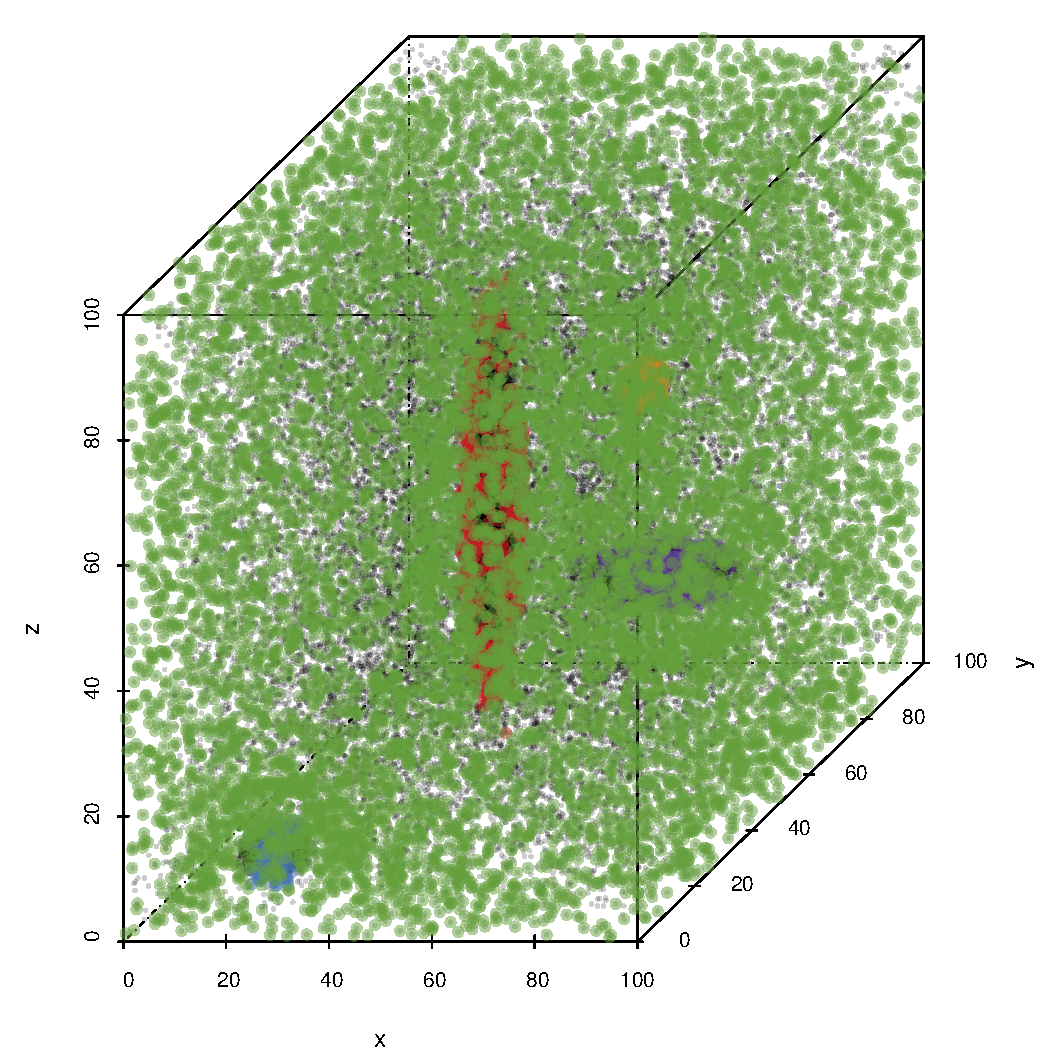
\includegraphics[keepaspectratio=true, width=\textwidth, height=0.23\textheight]{discussion/img/baakman_3_60000_anisotropy.png}
			\caption{Dataset \baakmanThree}
			\label{fig:discussion:anisotropy:baakman3}
		\end{subfigure}			
		\caption{Scatter plot of datasets
			\subref{fig:discussion:anisotropy:ferdosi2} \ferdosiTwo, %
			\subref{fig:discussion:anisotropy:baakman2} \baakmanTwo, %
			\subref{fig:discussion:anisotropy:ferdosi3} \ferdosiThree, and %
			\subref{fig:discussion:anisotropy:baakman3} \baakmanThree. %
			The points that have an anisotropy in the \nth{90} percentile are shown larger and in the color of the component they were drawn from.}
		\label{fig:discussion:anisotropy:multisphere}
	\end{figure}	